\documentclass[12pt,a4paper]{article}

\usepackage[T1]{fontenc}
\usepackage[utf8]{inputenc}
\usepackage{lmodern}
\usepackage[a4paper,margin=1in]{geometry}
\usepackage{setspace}
\usepackage{titlesec}
\usepackage{graphicx}
\usepackage{booktabs}
\usepackage{array}
\usepackage{tabularx}
\usepackage{longtable}
\usepackage{enumitem}
\usepackage{hyperref}
\usepackage{xcolor}
\usepackage{float}
\usepackage{listings}
\usepackage{tikz}
\usepackage{caption}
\usepackage{fancyhdr}

\usetikzlibrary{arrows.meta,positioning,shapes.geometric,fit,calc}

\onehalfspacing
\setlength{\parindent}{0pt}
\setlength{\parskip}{0.5em}
\setlist{leftmargin=1.4em}
\setcounter{secnumdepth}{3}
\setcounter{tocdepth}{3}

\renewcommand{\contentsname}{TABLE OF CONTENTS}

\hypersetup{
    colorlinks=true,
    linkcolor=black,
    urlcolor=blue
}

\newcolumntype{L}[1]{>{\raggedright\arraybackslash}p{#1}}
\newcolumntype{Y}{>{\raggedright\arraybackslash}X}

\lstset{
    basicstyle=\ttfamily\small,
    breaklines=true,
    frame=single,
    columns=fullflexible,
    backgroundcolor=\color{black!3},
    showstringspaces=false
}

\titleformat{\section}{\normalfont\bfseries\large}{\thesection.}{0.6em}{}
\titleformat{\subsection}{\normalfont\bfseries}{\thesubsection}{0.6em}{}
\titleformat{\subsubsection}{\normalfont\bfseries}{\thesubsubsection}{0.6em}{}
\titlespacing*{\section}{0pt}{1.1em}{0.4em}
\titlespacing*{\subsection}{0pt}{0.9em}{0.3em}
\titlespacing*{\subsubsection}{0pt}{0.7em}{0.2em}

\pagestyle{fancy}
\fancyhf{}
\fancyfoot[C]{\thepage}
\renewcommand{\headrulewidth}{0pt}

\newcommand{\snapshotplaceholder}[2]{
\begin{figure}[H]
\centering
\fbox{
\begin{minipage}[c][0.72\textheight][c]{0.9\textwidth}
\centering
\Large #1\\[1em]
\normalsize #2
\end{minipage}
}
\end{figure}
}

\begin{document}

\begin{titlepage}
\begin{center}
\vspace*{1.8cm}
{\Large\textbf{CAPSTONE PROJECT REPORT}}\\[0.3cm]
{\large (Project Term January--May 2026)}\\[1.4cm]
{\Large\textbf{SCROPIDS}}\\[0.5cm]
{\large Multi-Tenant Cloud-Native Intrusion Detection Platform\\
with Scheduler-Driven Aggregation and LLM-Assisted Threat Triage}\\[1.4cm]

{\large Submitted by}\\[0.7cm]

{\large [Student Name 1] \hspace{0.5cm} Registration Number: [Registration Number 1]}\\[0.25cm]
{\large [Student Name 2] \hspace{0.5cm} Registration Number: [Registration Number 2]}\\[0.25cm]
{\large [Student Name 3] \hspace{0.5cm} Registration Number: [Registration Number 3]}\\[1cm]

{\large Project Group Number: [Project Group Number]}\\[0.2cm]
{\large Course Code: CSE439}\\[1.1cm]

{\large Under the Guidance of}\\[0.25cm]
{\large [Mentor Name]}\\[0.2cm]
{\large School of Computer Science and Engineering}\\[0.2cm]
{\large Lovely Professional University, Punjab}\\[0.2cm]
{\large Academic Year: 2025--2026}
\end{center}
\end{titlepage}

\pagenumbering{roman}
\setcounter{page}{2}

\section*{PAC Form}
\addcontentsline{toc}{section}{PAC Form}
\begin{center}
\fbox{
\begin{minipage}{0.9\textwidth}
\textbf{Department Form Placeholder}

\vspace{0.5em}
Insert the signed PAC form, evaluation sheet, or department-issued annexure here before final submission.
\end{minipage}
}
\end{center}

\clearpage
\section*{DECLARATION}
\addcontentsline{toc}{section}{DECLARATION}
We hereby declare that the project work entitled \textit{ScropIDS -- Multi-Tenant Cloud-Native Intrusion Detection Platform with Scheduler-Driven Aggregation and LLM-Assisted Threat Triage} is an authentic record of our own work carried out as a requirement of the Capstone Project for the award of B.Tech degree in Computer Science / Data Science. All information furnished in this report is based on our own study, implementation, testing, technical analysis, and documentation. No part of this work has been submitted elsewhere for any other degree or diploma.

\vspace{0.8cm}
Name of Student 1: [Student Name 1] \hspace{0.4cm} Signature: \hrulefill

\vspace{0.5cm}
Name of Student 2: [Student Name 2] \hspace{0.4cm} Signature: \hrulefill

\vspace{0.5cm}
Name of Student 3: [Student Name 3] \hspace{0.4cm} Signature: \hrulefill

\vspace{0.5cm}
Date: \hrulefill

\clearpage
\section*{CERTIFICATE}
\addcontentsline{toc}{section}{CERTIFICATE}
This is to certify that the declaration statement made by the students for the project entitled \textit{ScropIDS -- Multi-Tenant Cloud-Native Intrusion Detection Platform with Scheduler-Driven Aggregation and LLM-Assisted Threat Triage} is correct to the best of my knowledge and belief. The work has been completed under my guidance and supervision. The present work is the result of original investigation, engineering effort, and academic study. No part of the work has been submitted earlier for any other degree. The project is fit for submission towards the capstone project requirement.

\vspace{1cm}
Signature and Name of the Mentor: [Mentor Name]\\
Designation: [Designation]\\
School of Computer Science and Engineering\\
Lovely Professional University, Punjab\\
Date: \hrulefill

\clearpage
\section*{ACKNOWLEDGEMENT}
\addcontentsline{toc}{section}{ACKNOWLEDGEMENT}
The successful completion of this project would not have been possible without the support, guidance, and encouragement of many people. We express our sincere gratitude to our project mentor for continual technical guidance, academic direction, and valuable suggestions throughout the lifecycle of this work.

We also acknowledge the broader open-source communities behind Django, Django REST Framework, React, Vite, Tailwind CSS, PostgreSQL, Redis, Celery, Go, and Docker. Their tools, documentation, and ecosystem support made it possible to design a practical platform that moves beyond theoretical problem discussion into a working implementation.

We further thank our peers, reviewers, and well-wishers who provided suggestions during the stages of architecture design, implementation, testing, and report preparation. Their feedback contributed to the improvement of both the technical depth and the usability of the project.

\clearpage
\tableofcontents
\clearpage
\pagenumbering{arabic}
\setcounter{page}{1}

\section*{1. INTRODUCTION}
In the present era of digital transformation, organizations are collecting more endpoint and infrastructure telemetry than ever before, yet many teams still struggle to turn that raw data into usable security decisions. Large enterprises often deploy combinations of SIEM, EDR, and rule-based monitoring platforms, but smaller security teams, academic labs, and emerging SaaS providers are frequently left with fragmented tools that are difficult to operate, expensive to scale, or limited in multi-tenant flexibility.

ScropIDS addresses this gap by proposing a multi-tenant cloud-native intrusion detection platform designed to simplify the journey from endpoint telemetry to analyst action. Instead of forcing users to manually correlate raw logs from several hosts, the platform accepts normalized JSON events from endpoint agents, stores them in a tenant-scoped backend, aggregates them into meaningful windows, evaluates those windows using rules and optional large language model assistance, and then surfaces actionable alerts through a centralized web interface.

From an implementation perspective, ScropIDS is built as a full-stack distributed platform. The backend is implemented with Django and Django REST Framework, background scheduling is handled through Celery and Redis, persistent storage is managed using PostgreSQL, the dashboard is built with React + Vite + TypeScript, and the endpoint agent is written in Go for cross-platform packaging. The project therefore combines software engineering, security operations, and cloud-native deployment ideas within a single capstone system.

This report presents the full technical narrative of ScropIDS. It discusses the problem context, rationale, feasibility, software requirements, architecture, design diagrams, implementation approach, testing, deployment, maintenance, and future roadmap. It also preserves the academic report structure expected by the reference capstone template while replacing its content with the actual features and workflow of the present project.

\setcounter{section}{1}

\clearpage
\section{PROFILE OF THE PROBLEM, RATIONALE \& SCOPE OF THE STUDY}

\subsection{Profile of the Problem}
Modern organizations generate an enormous amount of endpoint activity data from workstations, servers, and virtual machines. Suspicious process execution, repeated authentication failures, outbound beaconing, unusual file activity, and other warning signs often appear first at the endpoint level. However, in practice, this telemetry is usually scattered across local tools, inconsistent logs, and manual review processes.

In many small or medium-scale environments, analysts do not have a single structured system that can answer essential questions quickly. They may struggle to determine which endpoint is producing the most suspicious activity, whether similar signals are repeating across multiple hosts, or whether a particular stream of events is benign operational noise or a meaningful threat pattern. This leads to delayed triage, incomplete visibility, and a high likelihood of alert fatigue.

The problem becomes even more challenging in a multi-tenant environment. A shared platform must maintain strong tenant isolation while still offering central administration, secure agent enrollment, customizable detection policy, and usable analyst workflows. If tenancy is treated as an afterthought rather than a core design requirement, the risk of data leakage or operational confusion increases significantly.

Observation of existing practical workflows suggests several structural shortcomings:

\begin{enumerate}
    \item \textbf{Lack of Unified Telemetry Intake:} Endpoint events are often distributed across scripts, host-native tools, or manually collected logs rather than normalized into a consistent pipeline.
    \item \textbf{High Analyst Overhead:} Analysts are forced to inspect raw log records instead of consuming summarized, prioritized, and explainable signals.
    \item \textbf{Poor Tenant-Aware Controls:} Shared systems frequently lack clear tenant boundaries, configurable organization scoping, or per-tenant onboarding workflows.
    \item \textbf{Weak Operational Packaging:} Even when good detection logic exists, onboarding endpoint agents and synchronizing configuration remains cumbersome.
    \item \textbf{Inconsistent Explainability:} Alerts may exist, but the reasoning and recommended next steps are often missing or too generic to be useful.
    \item \textbf{Limited Adaptability:} Organizations with different budgets or privacy policies may want API-hosted AI models, local models, or no AI dependency at all, but existing workflows often support only one mode.
\end{enumerate}

These shortcomings indicate a strong need for a platform that combines endpoint telemetry collection, secure ingestion, scheduler-controlled aggregation, rule-based escalation, optional LLM-assisted reasoning, and multi-tenant dashboard access within a single consistent operational model.

\subsection{Rationale}
The rationale behind ScropIDS is both practical and academic. Practically, the project addresses the recurring difficulty of building a usable intrusion detection workflow out of scattered components. Many tools can collect logs, and many tools can display dashboards, but far fewer systems combine secure tenant onboarding, endpoint packaging, background aggregation, explainable triage, and configuration management in a single lightweight platform.

Academically, the project is valuable because it brings together multiple important domains of modern computing: systems programming through the Go agent, web application engineering through Django and React, asynchronous processing through Celery, data modeling through PostgreSQL, secure secret handling, multi-tenant access control, and machine-assisted decision support using strict JSON-based LLM outputs.

Another important rationale is flexibility. Some organizations may prefer OpenAI-compatible APIs for easier deployment, while others may require local inference through Ollama for cost, privacy, or offline operation. ScropIDS intentionally supports both. This makes the project more useful as a real engineering artifact rather than a narrow one-off demonstration.

The platform also reflects a usability-centered viewpoint. Intrusion detection is not only about generating alerts; it is about enabling analysts and administrators to understand the context of those alerts. By pairing aggregation windows, rule escalation, and human-readable reasoning, ScropIDS attempts to reduce the gap between raw telemetry and operational action.

\subsection{Scope of the Study}
The present study covers the design, implementation, and documentation of a production-oriented IDS platform with the following scope:

\begin{itemize}
    \item Cross-platform endpoint agent onboarding and event submission.
    \item Tenant-aware backend design using organizations, memberships, and scoped data ownership.
    \item Secure enrollment using one-time tokens and organization access tokens.
    \item Event ingestion, normalization, persistence, and scheduled aggregation.
    \item Rule-assisted and LLM-assisted threat analysis using validated JSON outputs.
    \item Alert queue generation and dashboard-driven analyst workflows.
    \item Operational configuration pages for LLM providers, scheduler settings, and escalation rules.
    \item Docker Compose deployment for reproducible local or pilot-scale environments.
\end{itemize}

The study does not attempt to deliver a full commercial EDR suite with kernel-level telemetry, enterprise-scale policy engines, advanced threat intelligence fusion, or complete incident response orchestration. Instead, it focuses on building a strong and extensible foundation that demonstrates technical depth, operational relevance, and future viability.

\subsection{Problem Statement}
The core problem addressed by this project is the absence of a unified, multi-tenant, cloud-native platform that can securely enroll endpoint agents, collect structured telemetry, aggregate suspicious activity, produce explainable threat assessments, and present those assessments to users through a central web console.

ScropIDS solves this problem by combining secure agent-to-cloud communication, tenant-aware backend architecture, scheduler-driven event grouping, configurable rules, optional LLM analysis, and dashboard-based operations. The resulting platform is intended to reduce analyst overhead, improve explainability, and create a more practical IDS workflow for academic, pilot, and small-scale operational use.

\clearpage
\section{EXISTING SYSTEM}

\subsection{Introduction}
Existing security monitoring practices generally fall into several recognizable categories: open-source host-based IDS tools, broad SIEM platforms, commercial endpoint detection products, and manual log review workflows. Each category contributes useful capabilities, but none of them perfectly matches the combined requirements of a multi-tenant, explainable, cloud-native platform that is both academically manageable and operationally meaningful.

The purpose of this section is not to dismiss existing solutions, but to establish a realistic baseline against which ScropIDS can be positioned. By understanding what current systems do well and where they become difficult to adapt, it becomes easier to justify the design choices in the proposed platform.

\subsection{Existing Software Analysis}
The following solutions represent the most relevant reference points for comparing the novelty and utility of ScropIDS.

\subsubsection{Wazuh / OSSEC}
Wazuh and OSSEC are well-known host-based intrusion detection platforms that provide agent-based monitoring, log collection, file integrity checks, and rule-driven alerting. They are respected within the open-source security community because they offer broad visibility without immediately forcing adoption of expensive commercial products.

However, their default operating model is not primarily optimized for lightweight multi-tenant SaaS delivery with highly customized tenant-specific dashboard workflows. While they are extensible and powerful, integrating them into a fully tenant-aware product with custom onboarding tokens, per-tenant model providers, and application-native UI flows can require substantial additional engineering effort.

They therefore serve as valuable reference systems for telemetry collection and rule-driven detection, but they do not by themselves deliver the full experience ScropIDS is targeting.

\subsubsection{Splunk / Elastic Security}
SIEM-style platforms such as Splunk and Elastic Security offer large-scale ingestion, search, correlation, visualization, and alerting. They are strong options for mature security teams with the operational capacity to manage pipelines, detections, and dashboards at significant scale.

Their main trade-off is operational complexity. For many small environments, academic prototypes, or focused SaaS products, the cost, deployment overhead, and tuning burden of a full SIEM can outweigh its immediate benefits. ScropIDS borrows the idea of centralized visibility from this class of products, but pursues a narrower and more purpose-built architecture.

Another key difference is explainability and packaging. ScropIDS integrates agent enrollment, scheduler policy, LLM provider configuration, and downloadable artifacts directly into the platform, rather than assuming a separate operational ecosystem around the monitoring backend.

\subsubsection{Commercial EDR Platforms}
Commercial endpoint detection and response platforms, including widely deployed products such as Microsoft Defender for Endpoint and CrowdStrike Falcon, provide deep telemetry, threat intelligence, and polished incident response workflows. These platforms often excel in detection maturity and enterprise operability.

At the same time, they are closed systems with licensing, integration, and deployment assumptions that make them less suitable as transparent capstone platforms. Their internal logic and data flows are not always visible enough for academic evaluation, and their operational model is usually not something a student project can reconfigure end-to-end.

ScropIDS is not intended to outperform commercial EDR suites in raw feature breadth. Instead, it aims to demonstrate how a smaller but complete and extensible platform can be engineered around similar concerns: endpoint visibility, triage, alert explanation, secure onboarding, and analyst usability.

\subsubsection{Manual Log Review and Script-Based Monitoring}
In many smaller organizations, monitoring still relies on native operating system logs, ad-hoc shell scripts, and manual review by administrators. This approach can be inexpensive to start with, but it scales poorly and often provides little consistency in how data is interpreted.

Manual workflows also create a high risk of missed patterns. If one endpoint exhibits repeated failed logins while another exhibits suspicious encoded command execution, it can be difficult for a human operator to recognize the connection unless those signals are normalized and grouped automatically.

ScropIDS improves on this by turning manual, host-by-host observation into a structured ingest-aggregate-analyze-alert cycle.

\subsection{Data Flow Diagram: Existing System}
The existing manual or loosely integrated monitoring workflow is illustrated in Figure~\ref{fig:existing-dfd}. The figure emphasizes how endpoint activity is often reviewed only after being scattered into disconnected tools and informal analyst processes.

\begin{figure}[H]
\centering
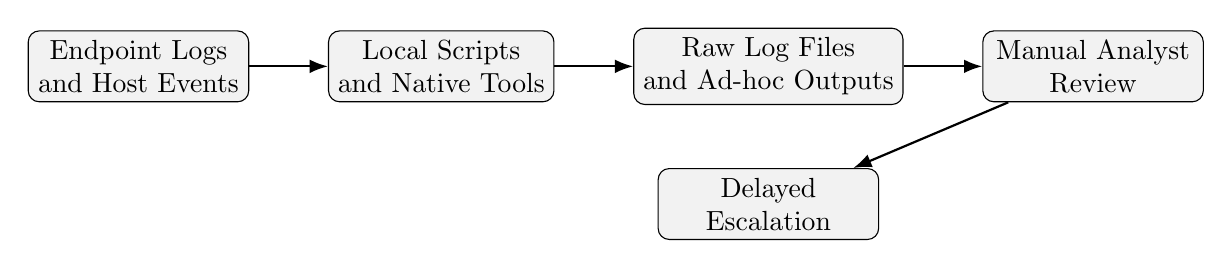
\begin{tikzpicture}[
node distance=8mm and 10mm,
box/.style={draw, rounded corners, minimum width=28mm, minimum height=9mm, align=center, fill=gray!10},
arr/.style={-Latex, thick}
]
\node[box] (endpoints) {Endpoint Logs\\and Host Events};
\node[box, right=of endpoints] (tools) {Local Scripts\\and Native Tools};
\node[box, right=of tools] (files) {Raw Log Files\\and Ad-hoc Outputs};
\node[box, right=of files] (analyst) {Manual Analyst\\Review};
\node[box, below=of files] (alert) {Delayed\\Escalation};

\draw[arr] (endpoints) -- (tools);
\draw[arr] (tools) -- (files);
\draw[arr] (files) -- (analyst);
\draw[arr] (analyst) -- (alert);
\end{tikzpicture}
\caption{Existing system data flow in a fragmented monitoring workflow.}
\label{fig:existing-dfd}
\end{figure}

\subsection{Innovations in the Proposed ScropIDS System}
ScropIDS introduces several innovations relative to the existing baseline:

\begin{itemize}
    \item \textbf{Tenant-aware platform design:} every core record is organization-scoped, supporting multi-tenant isolation from the start.
    \item \textbf{Structured onboarding:} both one-time enrollment tokens and organization access tokens are supported for safe agent registration.
    \item \textbf{Scheduler-driven aggregation:} raw events are grouped into analysis windows rather than being treated as isolated records only.
    \item \textbf{Hybrid triage model:} deterministic rules and validated LLM outputs cooperate rather than competing.
    \item \textbf{Cross-platform packaging:} downloadable artifacts are generated for multiple operating systems and architectures.
    \item \textbf{Integrated administration:} LLM configuration, scheduler settings, rules, alerts, and agent downloads are all available from the same platform.
\end{itemize}

Table~\ref{tab:existing-comparison} summarizes this comparison.

\begin{table}[H]
\centering
\begin{tabularx}{\textwidth}{L{3.2cm}L{5.6cm}Y}
\toprule
\textbf{Category} & \textbf{Common Limitation} & \textbf{ScropIDS Improvement} \\
\midrule
Manual monitoring & Slow correlation and high analyst effort & Automated aggregation and alert queue \\
Traditional HIDS & Limited product-style tenant workflows & Built-in tenant administration and onboarding \\
SIEM platforms & Heavy operational overhead & Lightweight focused deployment model \\
Commercial EDR & Closed ecosystem and low transparency & Extensible academic-friendly architecture \\
\bottomrule
\end{tabularx}
\caption{High-level comparison between existing approaches and ScropIDS.}
\label{tab:existing-comparison}
\end{table}

\clearpage
\section{PROBLEM ANALYSIS}

\subsection{Product Definition}
ScropIDS is a geospatially independent, cloud-native, multi-tenant intrusion detection platform designed to receive endpoint telemetry from distributed agents, transform that telemetry into meaningful aggregate windows, and generate alerts that analysts can understand and act upon.

At the core of the product is a separation between three perspectives:

\begin{itemize}
    \item \textbf{Endpoint perspective:} agents collect local host signals and submit them securely.
    \item \textbf{Platform perspective:} the backend stores, aggregates, analyzes, and prioritizes telemetry.
    \item \textbf{User perspective:} analysts and administrators interact with alerts, configurations, and onboarding workflows through the dashboard.
\end{itemize}

The product therefore sits at the intersection of endpoint monitoring, SaaS administration, and explainable threat analysis. It is not merely a log collector or a dashboard. It is an engineered workflow that connects enrollment, telemetry, aggregation, reasoning, and analyst action.

Table~\ref{tab:key-components} identifies the major components of the system.

\begin{table}[H]
\centering
\begin{tabularx}{\textwidth}{L{3.8cm}Y}
\toprule
\textbf{Component} & \textbf{Description} \\
\midrule
Endpoint Agent & Cross-platform Go binary for enrollment, heartbeat, event submission, and runtime sync \\
Secure Ingest API & Django REST endpoints for authenticated telemetry and tenant workflows \\
Tenant Model & Organization, membership, and scoped ownership model for data isolation \\
Aggregation Engine & Background scheduler logic that groups unprocessed events into windows \\
Rule Engine & Threshold and correlation-based escalation logic \\
LLM Layer & OpenAI-compatible or Ollama-backed analysis with strict JSON validation \\
Alert Queue & Tenant-scoped alert records with threat level, confidence, and reasoning \\
Web Dashboard & React interface for analysts and administrators \\
\bottomrule
\end{tabularx}
\caption{Key components of the ScropIDS platform.}
\label{tab:key-components}
\end{table}

\subsection{Feasibility Analysis}

\subsubsection{Technical Feasibility}
The system is technically feasible because it is built with widely adopted technologies that are well matched to the problem. Django REST Framework provides a stable API layer, PostgreSQL offers robust relational storage with JSON support, Redis and Celery enable periodic background execution, React + Vite support a responsive frontend, and Go provides an efficient path for cross-platform agent compilation.

The repository already contains concrete implementations for organizations, agent authentication, event ingestion, aggregation windows, alert storage, scheduler profiles, LLM provider management, and dashboard pages. This means the project has moved beyond conceptual design into working system construction.

The modularity of the codebase also improves technical feasibility. The agent, backend, frontend, and documentation are clearly separated, which makes maintenance and extension more manageable.

\subsubsection{Economic Feasibility}
From an economic perspective, ScropIDS is viable because its primary technology stack is open source. A local deployment can be executed using community-supported runtimes without mandatory licensing costs. This is important for academic work and small pilot environments.

The platform also gives operators control over inference cost. Tenants can configure paid API-hosted providers or choose local inference through Ollama. That flexibility makes the solution more realistic for environments with budget constraints or data sovereignty concerns.

Operationally, the use of Docker Compose reduces setup friction and shortens the path from development to demonstration. This lowers the total cost of experimentation and adoption.

\subsubsection{Operational Feasibility}
Operational feasibility depends on whether real users can actually manage and benefit from the system. ScropIDS has been designed so that administrators can create organizations, rotate tokens, manage providers, edit scheduler rules, and review alerts from one dashboard instead of across several disconnected tools.

The agent enrollment experience is also operationally feasible because it supports both interactive setup and environment-variable-based execution. This allows it to fit classroom demos, test labs, or semi-automated rollout scenarios.

The presence of documented smoke-test flows further supports operational feasibility, because deployment verification can be repeated in a structured manner.

\subsubsection{Time Feasibility}
The project is time-feasible within a capstone schedule because the implementation can be approached in phases. The system architecture allows early progress on backend models and APIs, followed by dashboard workflows, agent onboarding, testing, and documentation.

This staged approach reduces dependency bottlenecks. For example, the dashboard can be built against a stable API contract while the agent packaging workflow is still being refined. Similarly, the scheduler and rule engine can function before advanced LLM tuning is complete.

Time feasibility is therefore improved by modular decomposition and by the clear separation between core functionality and future enhancements.

\subsubsection{Legal and Ethical Feasibility}
Intrusion detection inevitably involves the processing of sensitive system data. For that reason, any deployment of ScropIDS must be authorized by the organization operating the monitored endpoints. Consent, policy compliance, and data minimization are critical.

The design of ScropIDS supports legal and ethical feasibility by treating LLM output as advisory, encrypting provider secrets at rest, requiring authenticated agent communication, and preserving tenant boundaries. These measures do not eliminate all risk, but they demonstrate responsible engineering choices.

Because the project is intended for academic and controlled deployment contexts, ethical feasibility also depends on transparency. The platform should clearly communicate what data it collects, how it stores it, and how administrators can control access.

\subsection{Project Plan}
The project was organized as a staged engineering effort, shown in Table~\ref{tab:project-plan}.

\begin{table}[H]
\centering
\begin{tabularx}{\textwidth}{L{2.2cm}Y Y}
\toprule
\textbf{Phase} & \textbf{Primary Activities} & \textbf{Key Outcome} \\
\midrule
Phase 1 & Problem analysis, literature study, and system scoping & Clear project direction \\
Phase 2 & Tenancy model, architecture, and API contract design & Design foundation established \\
Phase 3 & Backend implementation for organizations, agents, ingest, and alerts & Core service layer operational \\
Phase 4 & Frontend implementation for overview, alerts, agents, rules, and scheduler & Usable operational dashboard \\
Phase 5 & Go agent onboarding, packaging, and runtime profile synchronization & End-to-end telemetry workflow enabled \\
Phase 6 & Testing, documentation, report preparation, and refinement & Submission-ready capstone deliverables \\
\bottomrule
\end{tabularx}
\caption{Project plan used for the staged execution of ScropIDS.}
\label{tab:project-plan}
\end{table}

\clearpage
\section{SOFTWARE REQUIREMENT ANALYSIS}

\subsection{Introduction}
Software requirement analysis defines what the system must do, how different users interact with it, and what quality constraints it must satisfy. In ScropIDS, this analysis is particularly important because the platform supports both human users and machine agents. Human users need visibility, control, and safety; agents need a stable, secure, and low-friction communication pathway.

The requirement analysis also reflects the multi-tenant nature of the project. Requirements are not only about detection logic; they are also about isolation, configuration, explainability, and manageability.

\subsection{General Description}
The core actors in the system are summarized in Table~\ref{tab:actors}.

\begin{table}[H]
\centering
\begin{tabularx}{\textwidth}{L{4cm}Y}
\toprule
\textbf{Actor} & \textbf{Role in the System} \\
\midrule
Platform Administrator & Manages users, organizations, and operational setup at a broader level \\
Tenant Owner / Admin & Creates tokens, configures providers, tunes rules, and supervises tenant operations \\
Security Analyst & Reviews alerts, interprets reasoning, and updates alert status based on investigations \\
Endpoint Agent & Enrolls with backend, syncs runtime profile, sends events, and sends heartbeat signals \\
\bottomrule
\end{tabularx}
\caption{Primary actors in the ScropIDS platform.}
\label{tab:actors}
\end{table}

\subsection{Specific Requirements}

\subsubsection{Functional Requirements}
The functional requirements of ScropIDS are grouped below.

\textbf{Tenant and User Management}
\begin{itemize}
    \item FR1: The system shall support creation of tenant organizations.
    \item FR2: The system shall maintain organization memberships with role-specific access.
    \item FR3: The system shall allow dashboard users to authenticate using session-based login.
\end{itemize}

\textbf{Agent Enrollment and Endpoint Operations}
\begin{itemize}
    \item FR4: The system shall issue one-time enrollment tokens for controlled onboarding.
    \item FR5: The system shall provide organization access tokens for faster bulk-style enrollment.
    \item FR6: The system shall generate unique \texttt{agent\_id} and \texttt{agent\_token} values for enrolled endpoints.
    \item FR7: The agent shall send heartbeat messages and event batches to the backend.
    \item FR8: The agent shall retrieve runtime scheduler configuration from the backend.
\end{itemize}

\textbf{Telemetry and Analysis}
\begin{itemize}
    \item FR9: The backend shall ingest normalized event JSON and store tenant-scoped records.
    \item FR10: The scheduler shall aggregate unprocessed events by organization and agent.
    \item FR11: The system shall support rule-based escalation over aggregate summaries.
    \item FR12: The system shall support LLM-assisted analysis using active tenant-specific providers.
    \item FR13: The platform shall create alerts when the resulting threat level crosses the configured threshold.
\end{itemize}

\textbf{Dashboard and Administration}
\begin{itemize}
    \item FR14: The dashboard shall provide overview metrics including agents, events, and active alerts.
    \item FR15: The dashboard shall provide an alert queue with detailed reasoning and recommended actions.
    \item FR16: The dashboard shall provide an agents page with package downloads and token workflows.
    \item FR17: The dashboard shall provide pages for LLM provider configuration, scheduler tuning, and rule management.
\end{itemize}

\subsubsection{Non-Functional Requirements}
\textbf{Performance}
\begin{itemize}
    \item NFR1: Routine dashboard queries should be responsive under ordinary tenant load.
    \item NFR2: Event batches should be accepted efficiently enough to support frequent agent submissions.
    \item NFR3: Scheduled aggregation should execute predictably based on the configured interval.
\end{itemize}

\textbf{Security}
\begin{itemize}
    \item NFR4: Tenant records must remain isolated by organization ownership.
    \item NFR5: Agent authentication must be enforced on ingest and runtime config endpoints.
    \item NFR6: Provider API keys must be encrypted at rest.
    \item NFR7: LLM output must be validated before it is treated as an analysis result.
\end{itemize}

\textbf{Reliability and Maintainability}
\begin{itemize}
    \item NFR8: The system should remain operable even if an LLM provider is unavailable.
    \item NFR9: The codebase should remain modular enough to support future collectors and rules.
    \item NFR10: The platform should be reproducible using documented setup steps and containerized services.
\end{itemize}

\textbf{Usability}
\begin{itemize}
    \item NFR11: The UI should present alerts in a way that is understandable to analysts.
    \item NFR12: Administrative controls should be accessible from a centralized dashboard rather than scattered across separate tools.
\end{itemize}

\clearpage
\section{DESIGN}

\subsection{System Architecture}
The system architecture of ScropIDS is shown in Figure~\ref{fig:architecture}. It emphasizes the end-to-end flow from endpoints to analysts. The design is intentionally layered so that data collection, ingest, storage, background processing, model-assisted analysis, and user interaction can evolve independently while remaining operationally connected.

\begin{figure}[H]
\centering
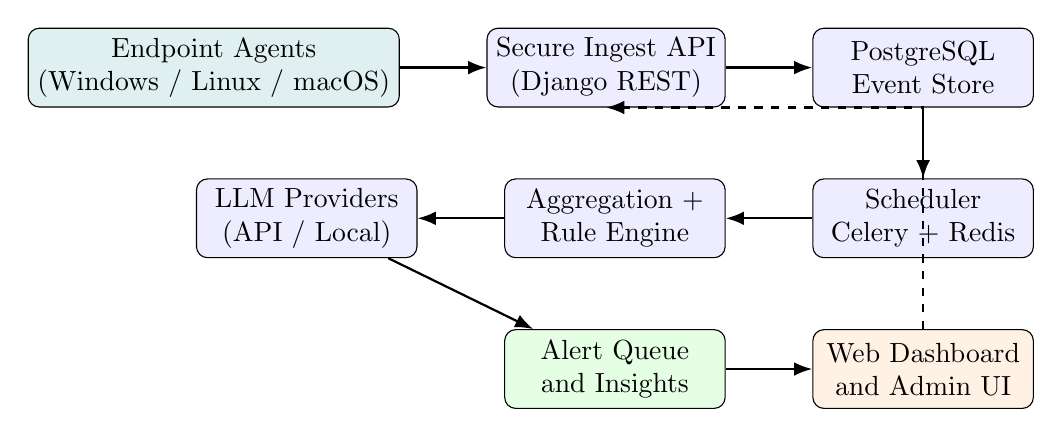
\begin{tikzpicture}[
node distance=9mm and 11mm,
box/.style={draw, rounded corners, minimum width=28mm, minimum height=10mm, align=center, fill=blue!7},
arr/.style={-Latex, thick}
]
\node[box, fill=teal!12] (agent) {Endpoint Agents\\(Windows / Linux / macOS)};
\node[box, right=of agent] (api) {Secure Ingest API\\(Django REST)};
\node[box, right=of api] (db) {PostgreSQL\\Event Store};
\node[box, below=of db] (sched) {Scheduler\\Celery + Redis};
\node[box, left=of sched] (agg) {Aggregation +\\Rule Engine};
\node[box, left=of agg] (llm) {LLM Providers\\(API / Local)};
\node[box, below=of agg, fill=green!10] (alerts) {Alert Queue\\and Insights};
\node[box, right=of alerts, fill=orange!10] (ui) {Web Dashboard\\and Admin UI};

\draw[arr] (agent) -- (api);
\draw[arr] (api) -- (db);
\draw[arr] (db) -- (sched);
\draw[arr] (sched) -- (agg);
\draw[arr] (agg) -- (llm);
\draw[arr] (llm) -- (alerts);
\draw[arr] (alerts) -- (ui);
\draw[arr, dashed] (ui.north) |- (api.south);
\end{tikzpicture}
\caption{High-level system architecture of ScropIDS.}
\label{fig:architecture}
\end{figure}

At the architectural level, the platform has four especially important characteristics:

\begin{itemize}
    \item it separates endpoint behavior from backend processing,
    \item it keeps tenant ownership as a first-class data property,
    \item it treats scheduled aggregation as central rather than optional,
    \item it presents alerts to human users only after they have been structured and prioritized.
\end{itemize}

\subsection{Design Notations}

\subsubsection{Data Flow Diagrams (DFD)}
Figure~\ref{fig:dfd-level0} presents a context-level DFD in which the platform acts as a processing core between endpoint agents, tenant users, and persistent data stores. Figure~\ref{fig:dfd-level1} refines the internal flow to show ingestion, aggregation, rule/LLM analysis, and alert display.

\begin{figure}[H]
\centering
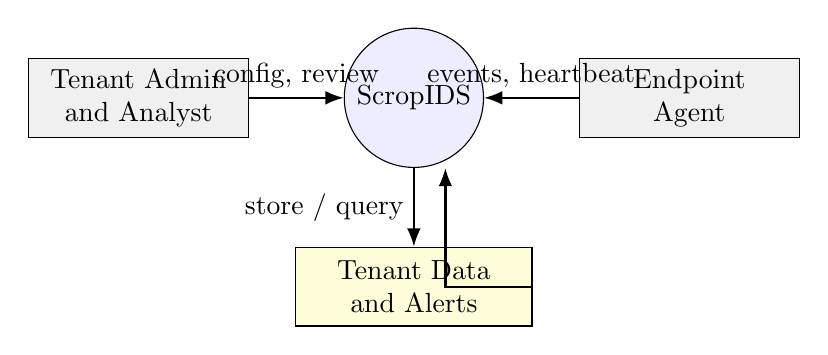
\begin{tikzpicture}[
node distance=10mm and 12mm,
ext/.style={draw, minimum width=28mm, minimum height=10mm, align=center, fill=gray!12},
proc/.style={draw, circle, minimum size=16mm, align=center, fill=blue!7},
data/.style={draw, minimum width=30mm, minimum height=10mm, align=center, fill=yellow!15},
arr/.style={-Latex, thick}
]
\node[ext] (tenant) {Tenant Admin\\and Analyst};
\node[proc, right=of tenant] (core) {ScropIDS};
\node[ext, right=of core] (agent) {Endpoint\\Agent};
\node[data, below=of core] (store) {Tenant Data\\and Alerts};

\draw[arr] (tenant) -- node[above]{config, review} (core);
\draw[arr] (agent) -- node[above]{events, heartbeat} (core);
\draw[arr] (core) -- node[left]{store / query} (store);
\draw[arr] (store.east) -| ($(core.south)+(0.4,0)$);
\end{tikzpicture}
\caption{DFD level 0 for ScropIDS.}
\label{fig:dfd-level0}
\end{figure}

\begin{figure}[H]
\centering
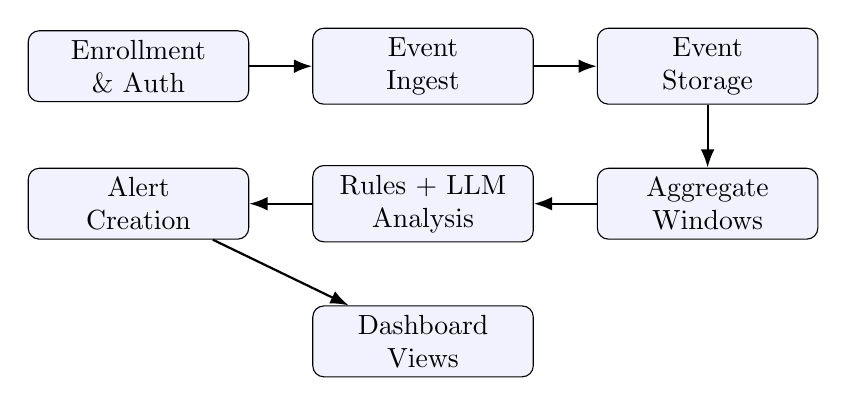
\begin{tikzpicture}[
node distance=8mm and 8mm,
box/.style={draw, rounded corners, minimum width=28mm, minimum height=9mm, align=center, fill=blue!5},
arr/.style={-Latex, thick}
]
\node[box] (enroll) {Enrollment\\\& Auth};
\node[box, right=of enroll] (ingest) {Event\\Ingest};
\node[box, right=of ingest] (eventdb) {Event\\Storage};
\node[box, below=of eventdb] (aggregate) {Aggregate\\Windows};
\node[box, left=of aggregate] (analysis) {Rules + LLM\\Analysis};
\node[box, left=of analysis] (alerts) {Alert\\Creation};
\node[box, below=of analysis] (dashboard) {Dashboard\\Views};

\draw[arr] (enroll) -- (ingest);
\draw[arr] (ingest) -- (eventdb);
\draw[arr] (eventdb) -- (aggregate);
\draw[arr] (aggregate) -- (analysis);
\draw[arr] (analysis) -- (alerts);
\draw[arr] (alerts) -- (dashboard);
\end{tikzpicture}
\caption{DFD level 1 showing the internal ScropIDS analysis flow.}
\label{fig:dfd-level1}
\end{figure}

\subsubsection{Entity Relationship Diagram}
The Entity Relationship Diagram in Figure~\ref{fig:erd} summarizes how tenant-aware data relationships are enforced throughout the system. The organization entity acts as the parent scope for memberships, agents, events, aggregated windows, alerts, scheduler profiles, and LLM provider settings.

\begin{figure}[H]
\centering
\resizebox{\textwidth}{!}{
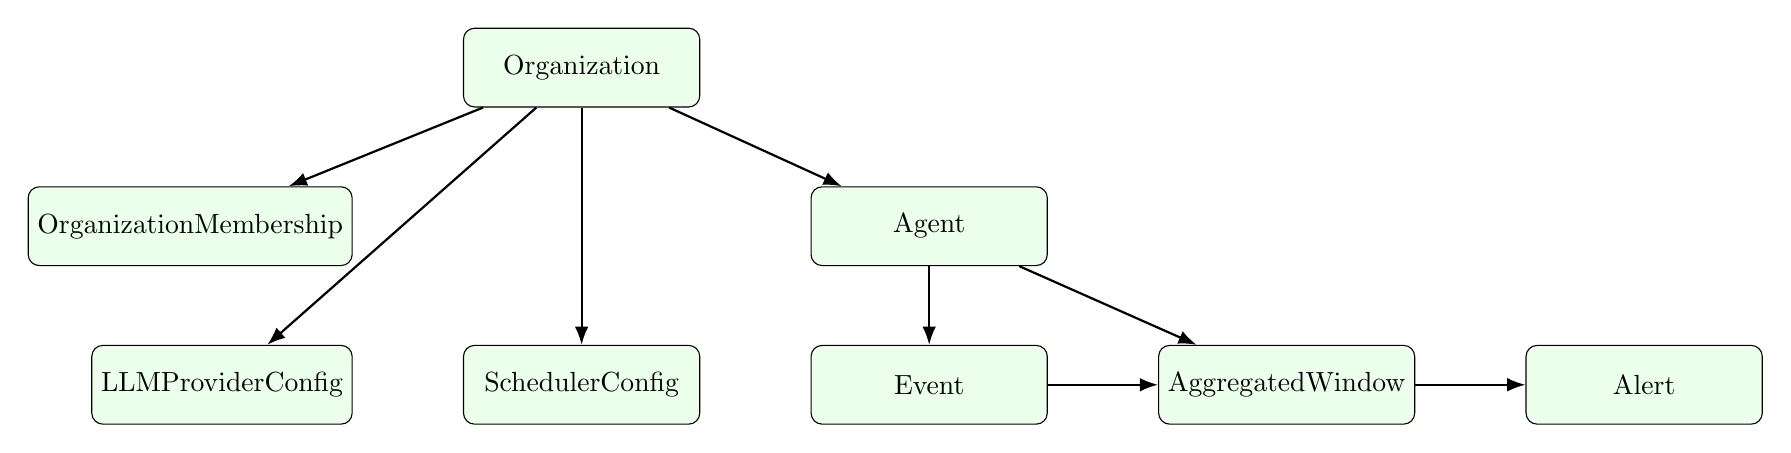
\begin{tikzpicture}[
node distance=10mm and 14mm,
ent/.style={draw, rounded corners, minimum width=30mm, minimum height=10mm, align=center, fill=green!8},
arr/.style={-Latex, thick}
]
\node[ent] (org) {Organization};
\node[ent, below left=of org] (member) {OrganizationMembership};
\node[ent, below right=of org] (agent) {Agent};
\node[ent, below=of agent] (event) {Event};
\node[ent, right=of event] (agg) {AggregatedWindow};
\node[ent, right=of agg] (alert) {Alert};
\node[ent, left=of event] (sched) {SchedulerConfig};
\node[ent, left=of sched] (llm) {LLMProviderConfig};

\draw[arr] (org) -- (member);
\draw[arr] (org) -- (agent);
\draw[arr] (org) -- (sched);
\draw[arr] (org) -- (llm);
\draw[arr] (agent) -- (event);
\draw[arr] (agent) -- (agg);
\draw[arr] (agg) -- (alert);
\draw[arr] (event) -- (agg);
\end{tikzpicture}
}
\caption{Simplified ER diagram of the ScropIDS data model.}
\label{fig:erd}
\end{figure}

\subsection{Detailed Module Design}

\subsubsection{Agent Enrollment and Collection Module}
This module is responsible for connecting endpoints to the platform. The Go agent supports interactive setup, direct credential mode, one-time enrollment token mode, and organization access token mode. After enrollment, it stores local configuration and periodically performs three tasks: refreshing runtime configuration, sending heartbeat messages, and transmitting event batches.

The collector design is intentionally modular. Current capabilities include process snapshots, security log sampling, network state snapshots, and system-status metadata. This layout leaves space for future file integrity and deeper operating-system-specific collectors without forcing a redesign of the enrollment logic.

\subsubsection{Secure Ingest and Tenancy Module}
The secure ingest module begins at the API boundary. It authenticates requests using agent headers, validates payload schemas, filters scaffold data where appropriate, and assigns every stored record to an organization. For human users, tenancy is resolved from session-authenticated membership data and an optional organization slug header.

This dual-authentication model is one of the strongest design features of the system because it recognizes that human and machine actors have fundamentally different operational identities. Analysts should not be authenticated like agents, and agents should not have the privileges of human users.

\subsubsection{Aggregation, Rule Engine, and Threat Analysis Module}
This module transforms raw telemetry into usable detection outputs. The scheduler identifies eligible unprocessed events, filters them based on configured minimum severity, groups them by organization and agent, and derives a summary payload. That payload includes counters such as failed logins, suspicious commands, new processes, and external connections.

The summary is then passed through the analysis pipeline. If an LLM provider is active, the platform requests a strict JSON threat assessment. After that, the rule engine evaluates built-in and custom threshold logic, possibly escalating the final threat level or confidence value. This hybrid design means that LLMs enhance the system rather than acting as its sole detection logic.

\subsubsection{Alerting, Dashboard, and Notification Module}
Once a final analyzed state is available, the platform checks whether the threat level exceeds the configured alert threshold. If it does, a tenant-scoped alert record is created. Alerts are then displayed in the dashboard, where analysts can review details, change status, and use recommended actions as decision support.

This module also encompasses operator-oriented pages for rules, scheduler profiles, provider configuration, and agent downloads. In this way, the same product supports both analysis and administration without separating them into unrelated interfaces.

\subsection{Flowcharts}

\subsubsection{Agent Enrollment Flowchart}
\begin{figure}[H]
\centering
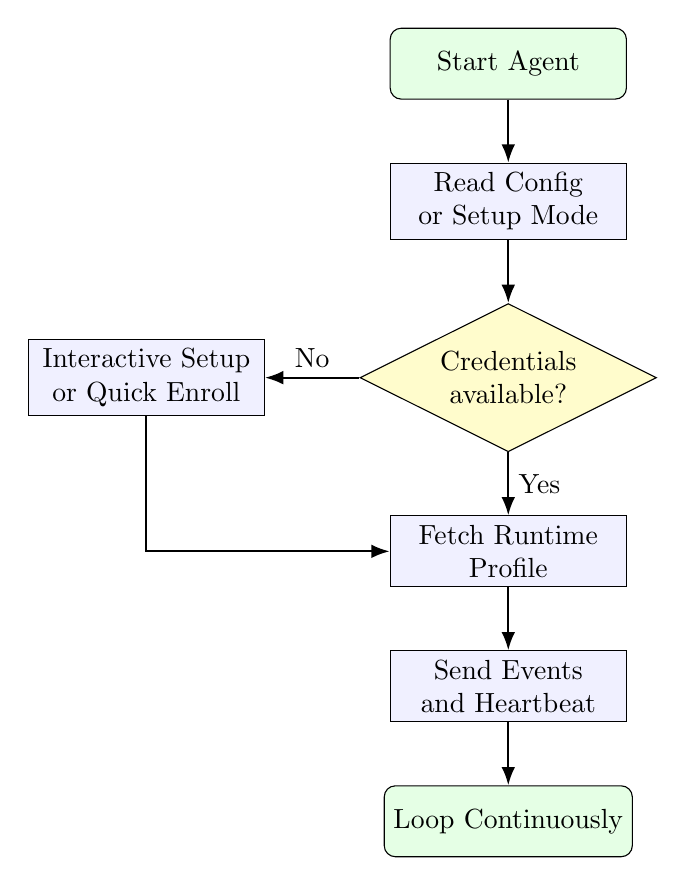
\begin{tikzpicture}[
node distance=8mm and 12mm,
term/.style={draw, rounded corners, minimum width=30mm, minimum height=9mm, align=center, fill=green!10},
proc/.style={draw, minimum width=30mm, minimum height=9mm, align=center, fill=blue!6},
dec/.style={draw, diamond, aspect=2, align=center, fill=yellow!20},
arr/.style={-Latex, thick}
]
\node[term] (start) {Start Agent};
\node[proc, below=of start] (mode) {Read Config\\or Setup Mode};
\node[dec, below=of mode] (hascred) {Credentials\\available?};
\node[proc, left=of hascred] (wizard) {Interactive Setup\\or Quick Enroll};
\node[proc, below=of hascred] (runtime) {Fetch Runtime\\Profile};
\node[proc, below=of runtime] (send) {Send Events\\and Heartbeat};
\node[term, below=of send] (end) {Loop Continuously};

\draw[arr] (start) -- (mode);
\draw[arr] (mode) -- (hascred);
\draw[arr] (hascred) -- node[above]{No} (wizard);
\draw[arr] (wizard) |- (runtime);
\draw[arr] (hascred) -- node[right]{Yes} (runtime);
\draw[arr] (runtime) -- (send);
\draw[arr] (send) -- (end);
\end{tikzpicture}
\caption{Flowchart for agent enrollment and runtime synchronization.}
\label{fig:agent-flow}
\end{figure}

\subsubsection{Alert Generation Flowchart}
\begin{figure}[H]
\centering
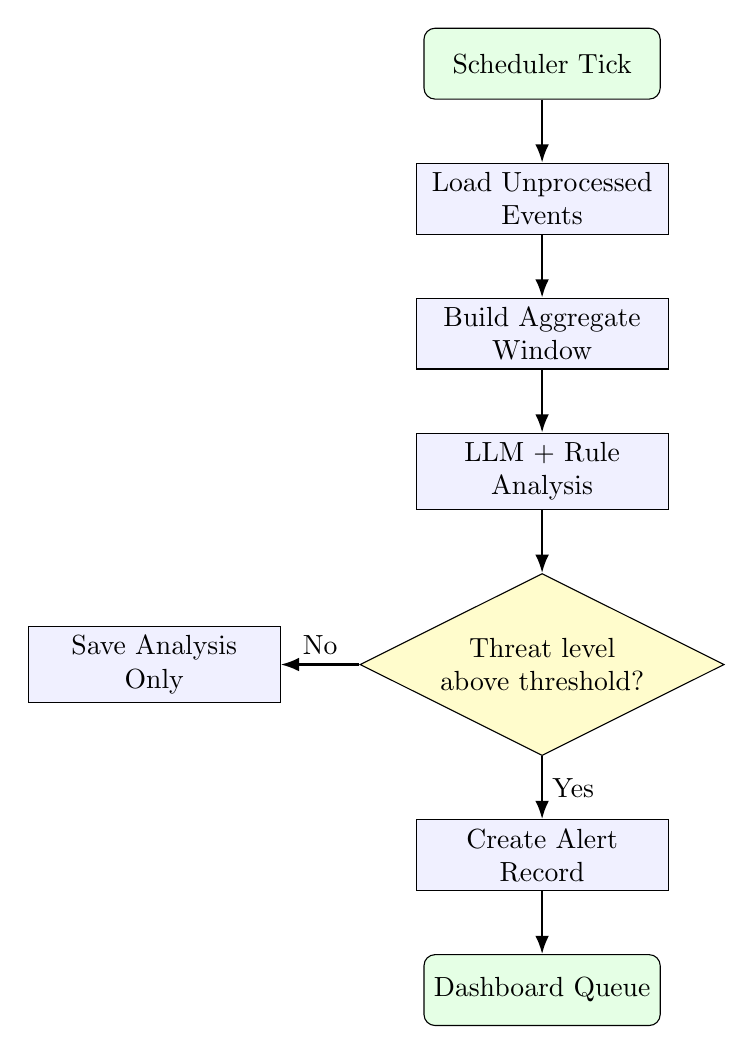
\begin{tikzpicture}[
node distance=8mm and 10mm,
term/.style={draw, rounded corners, minimum width=30mm, minimum height=9mm, align=center, fill=green!10},
proc/.style={draw, minimum width=32mm, minimum height=9mm, align=center, fill=blue!6},
dec/.style={draw, diamond, aspect=2, align=center, fill=yellow!20},
arr/.style={-Latex, thick}
]
\node[term] (start) {Scheduler Tick};
\node[proc, below=of start] (events) {Load Unprocessed\\Events};
\node[proc, below=of events] (aggregate) {Build Aggregate\\Window};
\node[proc, below=of aggregate] (analysis) {LLM + Rule\\Analysis};
\node[dec, below=of analysis] (threshold) {Threat level\\above threshold?};
\node[proc, left=of threshold] (save) {Save Analysis\\Only};
\node[proc, below=of threshold] (alert) {Create Alert\\Record};
\node[term, below=of alert] (end) {Dashboard Queue};

\draw[arr] (start) -- (events);
\draw[arr] (events) -- (aggregate);
\draw[arr] (aggregate) -- (analysis);
\draw[arr] (analysis) -- (threshold);
\draw[arr] (threshold) -- node[above]{No} (save);
\draw[arr] (threshold) -- node[right]{Yes} (alert);
\draw[arr] (alert) -- (end);
\end{tikzpicture}
\caption{Flowchart for alert generation from aggregated telemetry.}
\label{fig:alert-flow}
\end{figure}

\subsection{Pseudocode}

\subsubsection{Aggregation Algorithm}
\begin{lstlisting}
for each active scheduler profile:
    determine the current aggregation window
    fetch unprocessed tenant events
    filter events below minimum severity
    group events by agent
    for each group:
        derive summary counters
        create aggregated window record
    mark included events as processed
    analyze new windows
\end{lstlisting}

\subsubsection{Threat Escalation Algorithm}
\begin{lstlisting}
load llm_output and aggregate summary
set final_threat = llm_output.threat_level
set final_confidence = llm_output.confidence

for each enabled rule:
    if rule conditions match summary counters:
        final_threat = max(final_threat, rule.target_threat)
        final_confidence = max(final_confidence, rule.min_confidence)
        record rule match

if final_threat >= configured alert threshold:
    create alert
else:
    save analysis without alert creation
\end{lstlisting}

\clearpage
\section{TESTING}

\subsection{Functional Testing}
Functional testing focused on validating whether the major user-facing and agent-facing features behave as expected. Instead of checking only isolated functions, this level of testing verifies that the operational promise of the system is actually achieved.

Table~\ref{tab:functional-testing} summarizes the major functional test areas.

\begin{table}[H]
\centering
\begin{tabularx}{\textwidth}{L{3.3cm}Y Y}
\toprule
\textbf{Test Area} & \textbf{Purpose} & \textbf{Current Evidence} \\
\midrule
Backend unit tests & Validate token handling and aggregate processing logic & \texttt{./backend/.venv/bin/python manage.py test apps.core} \\
Frontend build & Verify the React dashboard compiles into a production bundle & \texttt{npm run build} \\
Go agent build & Verify cross-platform starter agent source compiles correctly & \texttt{go build -o /tmp/scropids-agent-verify ./cmd/agent} \\
SaaS smoke workflow & Validate create-tenant, enroll-agent, ingest, aggregate, and overview flow & Documented in \texttt{docs/smoke-test-saas.md} \\
Alert queue workflow & Validate alert creation, viewing, and status transitions & Verified through dashboard pages and API routes \\
\bottomrule
\end{tabularx}
\caption{Functional testing summary for ScropIDS.}
\label{tab:functional-testing}
\end{table}

\subsection{Structural Testing (White-Box Testing)}
Structural testing was used to evaluate internal correctness rather than only visible outcomes. This was especially important in parts of the platform where boundary behavior or conditional branching affects security and reliability.

The main components emphasized in structural testing were:

\begin{itemize}
    \item agent token round-trip validation,
    \item one-time token usability and expiry semantics,
    \item event aggregation and processed-state updates,
    \item rule threshold evaluation under edge conditions,
    \item JSON validation of LLM outputs,
    \item runtime configuration refresh behavior in the agent.
\end{itemize}

Table~\ref{tab:whitebox} summarizes representative white-box checks.

\begin{table}[H]
\centering
\begin{tabularx}{\textwidth}{L{3.8cm}L{4.8cm}Y}
\toprule
\textbf{Component} & \textbf{Testing Approach} & \textbf{Outcome} \\
\midrule
Agent token model methods & Valid and invalid token comparisons & Only correct tokens authenticate \\
Enrollment token lifecycle & Fresh, expired, and used-token scenarios & Single-use and expiry behavior preserved \\
Aggregation pipeline & Event insertion followed by aggregation window creation & Events marked processed after inclusion \\
Rule escalation logic & Controlled summary counters around thresholds & Escalation occurs only when conditions match \\
LLM schema validation & Missing keys, wrong types, and valid JSON payloads & Invalid output rejected, valid output accepted \\
\bottomrule
\end{tabularx}
\caption{Structural testing summary.}
\label{tab:whitebox}
\end{table}

\subsection{Levels of Testing}

\subsubsection{Unit Testing}
Unit testing verifies small isolated parts of the system. In the backend, this includes model methods, token checking behavior, and the aggregate creation process. These tests are especially important because they confirm correctness before components are wired together into full workflows.

For frontend components, the codebase structure also supports isolated rendering and view-level testing in future iterations. Although the current focus is on build validation and integrated behavior, the component design supports deeper UI unit testing later.

\subsubsection{Integration Testing}
Integration testing ensures that separate modules exchange data correctly. In ScropIDS, this includes the path from authentication to organization resolution, the path from agent enrollment to ingest permissions, the path from event storage to aggregation, and the path from analysis output to alert visibility in the dashboard.

The documented smoke test flow is especially useful here because it exercises the system across several module boundaries using realistic API requests instead of only internal test doubles.

\subsubsection{System Testing}
System testing treats the platform as a complete operational product. For ScropIDS, system testing includes starting the services through Docker Compose, accessing the dashboard through the browser, running authenticated API calls, triggering background analysis, and reviewing the resulting alert queue.

This level of testing validates not only code behavior, but also service topology, environment configuration, cross-service dependencies, and the user-visible result of the overall design.

\subsubsection{User Acceptance Testing (UAT)}
User acceptance testing is concerned with whether the platform is usable and understandable to its intended audience. For ScropIDS, the primary UAT scenarios are:

\begin{itemize}
    \item signing in and switching tenant context,
    \item understanding dashboard metrics,
    \item reading alert reasoning,
    \item downloading and onboarding agents,
    \item configuring providers and scheduler settings without confusion.
\end{itemize}

The main acceptance criterion is not just whether the system is functional, but whether users can confidently navigate it and interpret the alert outputs it generates.

\subsubsection{Performance Testing}
Although the current project phase emphasizes correctness and architecture more than large-scale benchmarking, performance remains a non-functional concern. The design anticipates horizontal scaling by separating ingestion, persistent storage, and background execution. Future performance testing will need to measure ingest throughput, scheduler latency, queue backlog behavior, dashboard responsiveness, and tenant isolation under concurrent load.

At the present stage, performance assurance comes primarily from architectural choices rather than full benchmark campaigns. Even so, the modular service topology already places the system on a reasonable path toward more advanced load testing.

\clearpage
\section{IMPLEMENTATION}

\subsection{Implementation of the Project}
The project is implemented as a monorepo with separate but coordinated backend, frontend, agent, and documentation areas. This structure supports parallel development while keeping the overall platform reproducible and consistent.

The backend is implemented in Django and Django REST Framework. It provides the data model, tenancy layer, agent authentication, organization workflows, ingest endpoints, alert APIs, and configuration APIs. Celery workers and beat processes are used to execute scheduler-controlled background analysis tasks.

The frontend is implemented using React + Vite + TypeScript. It contains the operational screens used by analysts and administrators, including overview metrics, alerts, agents, scheduler configuration, LLM provider management, and rules.

The endpoint agent is implemented in Go. It supports interactive setup, configuration persistence, quick enrollment, runtime schedule synchronization, and event submission. It can be packaged into multiple platform-specific artifacts, which are then exposed back to users through downloadable manifests.

Figure~\ref{fig:deployment-topology} shows the implementation topology as deployed via Docker Compose.

\begin{figure}[H]
\centering
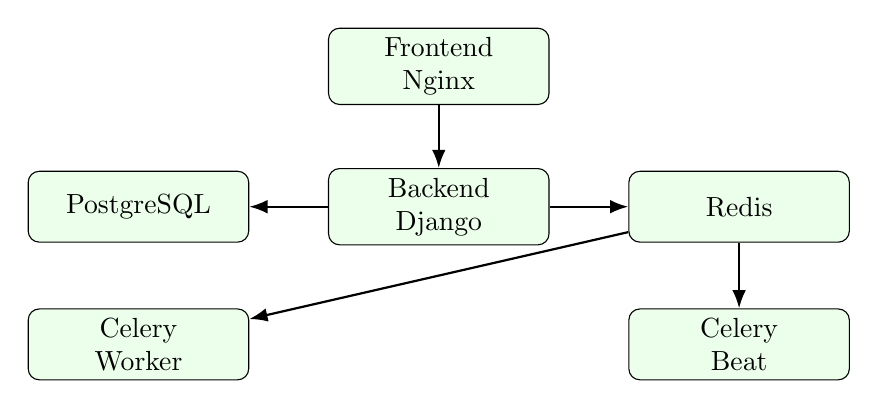
\begin{tikzpicture}[
node distance=8mm and 10mm,
box/.style={draw, rounded corners, minimum width=28mm, minimum height=9mm, align=center, fill=green!8},
arr/.style={-Latex, thick}
]
\node[box] (frontend) {Frontend\\Nginx};
\node[box, below=of frontend] (backend) {Backend\\Django};
\node[box, left=of backend] (postgres) {PostgreSQL};
\node[box, right=of backend] (redis) {Redis};
\node[box, below left=of backend] (worker) {Celery\\Worker};
\node[box, below right=of backend] (beat) {Celery\\Beat};

\draw[arr] (frontend) -- (backend);
\draw[arr] (backend) -- (postgres);
\draw[arr] (backend) -- (redis);
\draw[arr] (redis) -- (worker);
\draw[arr] (redis) -- (beat);
\end{tikzpicture}
\caption{Service topology used during implementation and deployment.}
\label{fig:deployment-topology}
\end{figure}

\subsection{Conversion Plan}
The deployment of ScropIDS into a real environment is best approached in phases. A phased conversion reduces risk, allows operator feedback to be collected early, and makes it easier to verify that tenant controls, agent enrollment, and analysis workflows behave correctly before a larger rollout.

Table~\ref{tab:conversion-plan} presents the phased conversion plan.

\begin{table}[H]
\centering
\begin{tabularx}{\textwidth}{L{1.2cm}Y}
\toprule
\textbf{Step} & \textbf{Description} \\
\midrule
1 & Prepare environment variables, database credentials, Redis connectivity, and backend secrets. \\
2 & Start the services and validate health checks for database, backend, worker, and frontend. \\
3 & Create an administrative user and at least one organization. \\
4 & Configure an LLM provider or deliberately validate the fallback no-provider path. \\
5 & Generate an enrollment token or rotate an organization access token. \\
6 & Enroll pilot agents and validate heartbeat plus event acceptance. \\
7 & Run scheduler ticks, review alert generation, and collect analyst feedback. \\
8 & Expand to broader endpoint coverage only after pilot validation is stable. \\
\bottomrule
\end{tabularx}
\caption{Phased conversion plan for ScropIDS deployment.}
\label{tab:conversion-plan}
\end{table}

\subsection{Post-Implementation and Software Maintenance}
After deployment, the platform must be maintained across several dimensions:

\begin{itemize}
    \item \textbf{Corrective Maintenance:} resolving bugs in authentication, ingest, scheduler behavior, or dashboard workflows.
    \item \textbf{Adaptive Maintenance:} updating external integrations such as model providers, packages, or infrastructure versions.
    \item \textbf{Perfective Maintenance:} improving UI clarity, detection quality, and performance based on operator feedback.
    \item \textbf{Preventive Maintenance:} patching dependencies, verifying backups, rotating tokens, and reviewing security posture proactively.
\end{itemize}

The maintenance cycle is illustrated in Figure~\ref{fig:maintenance-cycle}.

\begin{figure}[H]
\centering
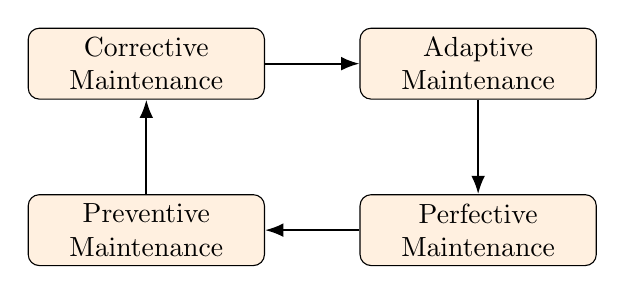
\begin{tikzpicture}[
node distance=12mm and 12mm,
box/.style={draw, rounded corners, minimum width=30mm, minimum height=9mm, align=center, fill=orange!12},
arr/.style={-Latex, thick}
]
\node[box] (corrective) {Corrective\\Maintenance};
\node[box, right=of corrective] (adaptive) {Adaptive\\Maintenance};
\node[box, below=of adaptive] (perfective) {Perfective\\Maintenance};
\node[box, left=of perfective] (preventive) {Preventive\\Maintenance};

\draw[arr] (corrective) -- (adaptive);
\draw[arr] (adaptive) -- (perfective);
\draw[arr] (perfective) -- (preventive);
\draw[arr] (preventive) -- (corrective);
\end{tikzpicture}
\caption{Maintenance cycle for the ongoing evolution of ScropIDS.}
\label{fig:maintenance-cycle}
\end{figure}

\clearpage
\section{PROJECT LEGACY}

\subsection{Current Status of the Project}
At the current stage, ScropIDS exists as a working capstone implementation rather than only a design proposal. The repository contains the backend data model, API routes, dashboard pages, agent starter, packaging scripts, and supporting documentation required to demonstrate the core workflow.

This means the project already supports a meaningful end-to-end scenario: create a tenant, enroll an agent, send telemetry, run aggregation, analyze an aggregate, create an alert, and review the result through a web interface. That level of completeness is an important marker of project maturity.

\subsection{Remaining Areas of Concern}
Despite its current maturity, several areas remain open for future hardening and refinement:

\begin{itemize}
    \item deeper OS-specific telemetry collectors are still needed,
    \item more extensive load and endurance testing should be conducted,
    \item role-based access control can be refined beyond the present baseline,
    \item threat intelligence enrichment and richer mapping to security frameworks remain future enhancements,
    \item long-term audit and observability features can be expanded further.
\end{itemize}

These concerns do not invalidate the present implementation; rather, they define the next layer of work needed to transition from a strong capstone system to a more production-ready security product.

\subsection{Technical and Managerial Lessons Learnt}

\subsubsection{Technical Lessons}
Several technical lessons emerged from this project. First, strict data contracts are extremely valuable: once telemetry is normalized and model output is forced into a validated JSON schema, downstream processing becomes much more reliable. Second, deterministic rules and model reasoning are stronger together than either approach alone; rules provide consistency, while model output improves explanation and prioritization.

Third, tenant isolation must be engineered into the data model at the beginning of the project rather than bolted on later. Finally, deployment and packaging are not secondary concerns. A security system that cannot be onboarded cleanly will struggle even if its detection logic is strong.

\subsubsection{Managerial Lessons}
From a managerial perspective, the project reinforced the importance of early requirement clarity and staged execution. Dividing the work into architecture, backend, frontend, agent, and validation phases reduced confusion and allowed progress to continue even when one component was still being refined.

The work also demonstrated the importance of documentation as part of development rather than after development. Architecture notes, API contracts, smoke test instructions, and report drafts made the project easier to validate and easier to explain.

Finally, iterative feedback was valuable. Small usability observations about the dashboard, token workflows, and wording of alerts had a large effect on the clarity of the final system.

\clearpage
\section{USER MANUAL (HELP GUIDE)}

\subsection{Introduction}
This section describes how intended users interact with ScropIDS. The platform serves three broad kinds of users: analysts who investigate alerts, tenant administrators who configure and onboard, and platform-level administrators who manage broader deployment concerns. It also serves endpoint agents, which function as authenticated machine actors.

\subsection{System Requirements}
\begin{table}[H]
\centering
\begin{tabularx}{\textwidth}{L{4cm}Y}
\toprule
\textbf{Component} & \textbf{Minimum Requirement} \\
\midrule
Backend Host & 2 vCPU, 4 GB RAM for pilot-scale deployment \\
Database & PostgreSQL 13+ with JSON-capable storage \\
Queue & Redis 6+ \\
Agent Endpoint & Network access to backend and sufficient permission to read host signals \\
Frontend & Modern browser such as Chromium, Firefox, or Safari \\
\bottomrule
\end{tabularx}
\caption{Baseline system requirements for ScropIDS.}
\label{tab:system-requirements}
\end{table}

\subsection{Dashboard / Analyst User Guide}

\subsubsection{Account Registration and Login}
Open the application and navigate to the login page. If the deployment supports self-registration, a user can create an account and initial organization through the registration flow. Otherwise, the user should log in using the credentials provided by the administrator.

After authentication, the top header allows the user to select the active tenant workspace. This step is important because all subsequent dashboard views, alerts, and configuration screens are scoped to the currently selected organization.

\subsubsection{Using the Overview and Alerts Workspace}
Once logged in, the user should begin on the Overview page. This screen provides a summary of total agents, recent event activity, active alerts, threat distribution, and other tenant-specific operational indicators.

To investigate suspicious activity, the user can open the Alerts page. Each alert displays threat level, confidence, host context, reasoning, and recommended action. The alert detail drawer gives a more readable explanation of why the system prioritized that event window.

\subsubsection{Downloading, Enrolling, and Monitoring Agents}
The Agents page provides three important capabilities. First, it shows the enrolled endpoints for the active tenant along with last-seen information. Second, it allows the administrator to rotate or copy the organization access token. Third, it exposes downloadable agent packages for multiple platforms and architectures.

After downloading the correct artifact, the operator can run the agent using interactive setup or environment variables. Once enrollment is complete, the endpoint should begin appearing in the dashboard and its heartbeat should update the last-seen field.

\subsubsection{Handling Alerts and Recommended Actions}
When reviewing alerts, users should treat the displayed reasoning and recommended action as guided decision support. The platform helps prioritize and explain signals, but final investigation and remediation decisions remain the responsibility of the human analyst.

Alerts can be moved through statuses such as \texttt{open}, \texttt{in\_progress}, and \texttt{resolved}. This helps teams distinguish newly raised issues from actively investigated or closed items.

\subsection{Tenant Administrator Guide}

\subsubsection{Organization Setup and Access Control}
Tenant administrators are responsible for ensuring that the correct users belong to the correct organization. This includes validating memberships, confirming role assignments, and making sure the active workspace in the dashboard matches the intended tenant before administrative actions are taken.

\subsubsection{Managing Agents, Packages, and LLM Providers}
Tenant administrators can rotate organization access tokens, distribute agent packages, and enroll endpoints. They also manage LLM providers through the LLM Config page, where each provider can be activated, edited, or removed. The ability to switch between API-hosted and local inference is especially useful during pilot operation and testing.

\subsubsection{Managing Scheduler, Rules, and Alerts}
The Scheduler page controls aggregation interval, minimum severity, alert threshold, and agent runtime collector settings. The Rules page controls built-in and custom escalation behavior. Administrators should tune these carefully, because they directly influence how noisy or conservative the alert queue becomes.

\subsection{Administrator Guide}
Platform administrators operate at a broader scope than tenant administrators. Their responsibilities include deployment readiness, account provisioning, infrastructure verification, health monitoring, and broader policy oversight. In classroom or project demonstration environments, this role may be combined with the mentor or system operator role.

An administrator should regularly confirm:

\begin{itemize}
    \item backend health endpoint availability,
    \item database and Redis connectivity,
    \item worker and beat service activity,
    \item integrity of environment variables and secrets,
    \item successful execution of migrations and static collection.
\end{itemize}

\subsection{Troubleshooting Guide}
\begin{itemize}
    \item If agent enrollment fails, verify the organization slug, token value, and API base URL.
    \item If the dashboard is empty, confirm the correct tenant is selected and the user belongs to that organization.
    \item If no alerts are generated, check scheduler status, provider configuration, and alert threshold rules.
    \item If runtime sync fails, validate agent credentials and the \texttt{/api/v1/ingest/config/} endpoint.
    \item If the frontend does not load expected data, confirm backend CORS/CSRF settings and session authentication status.
\end{itemize}

\clearpage
\section{SYSTEM SNAPSHOTS}

\subsection{System Snapshots}
This section is intentionally reserved for the final visual evidence of the project. Because the capstone report is intended to exceed 50 pages and provide strong demonstration support, the snapshot section contains several full-page placeholders that can be replaced with actual screenshots, terminal outputs, and evidence captures before final submission.

\clearpage
\textbf{Snapshot 1: Login Page}
\snapshotplaceholder{Login Page}{Insert the session-based login screen used by dashboard users.}

\clearpage
\textbf{Snapshot 2: Registration / First Workspace Setup}
\snapshotplaceholder{Registration / First Workspace Setup}{Insert the account registration or initial tenant creation screen.}

\clearpage
\textbf{Snapshot 3: Dashboard Hero Section}
\snapshotplaceholder{Dashboard Hero Section}{Insert the main overview hero area with live threat summary.}

\clearpage
\textbf{Snapshot 4: Dashboard KPI Cards}
\snapshotplaceholder{Dashboard KPI Cards}{Insert cards or metrics for agents, events, alerts, and pending aggregates.}

\clearpage
\textbf{Snapshot 5: Threat Distribution Chart}
\snapshotplaceholder{Threat Distribution Chart}{Insert the chart that summarizes alert severities or confidence patterns.}

\clearpage
\textbf{Snapshot 6: Recent Alerts Table}
\snapshotplaceholder{Recent Alerts Table}{Insert the live recent alerts table from the overview page.}

\clearpage
\textbf{Snapshot 7: Alerts Queue Page}
\snapshotplaceholder{Alerts Queue Page}{Insert the main alert queue with filters and statuses.}

\clearpage
\textbf{Snapshot 8: Alert Detail Drawer}
\snapshotplaceholder{Alert Detail Drawer}{Insert the expanded alert drawer showing reasoning and recommended action.}

\clearpage
\textbf{Snapshot 9: Agents Page}
\snapshotplaceholder{Agents Page}{Insert the enrolled agent list with hostnames and online state.}

\clearpage
\textbf{Snapshot 10: Token Rotation Panel}
\snapshotplaceholder{Token Rotation Panel}{Insert the organization access token view after reset or reveal.}

\clearpage
\textbf{Snapshot 11: Artifact Download Section}
\snapshotplaceholder{Artifact Download Section}{Insert the downloadable agent artifacts list.}

\clearpage
\textbf{Snapshot 12: Quick Run Command}
\snapshotplaceholder{Quick Run Command}{Insert the command block shown to operators when starting the agent.}

\clearpage
\textbf{Snapshot 13: Agent Timeline Page}
\snapshotplaceholder{Agent Timeline Page}{Insert the per-agent event and LLM insight history.}

\clearpage
\textbf{Snapshot 14: LLM Provider Overview}
\snapshotplaceholder{LLM Provider Overview}{Insert the list of configured LLM providers for a tenant.}

\clearpage
\textbf{Snapshot 15: LLM Provider Create / Edit Form}
\snapshotplaceholder{LLM Provider Create / Edit Form}{Insert the provider creation or edit form.}

\clearpage
\textbf{Snapshot 16: Scheduler Management Page}
\snapshotplaceholder{Scheduler Management Page}{Insert the scheduler controls for aggregation and agent runtime.}

\clearpage
\textbf{Snapshot 17: Rule Engine Page}
\snapshotplaceholder{Rule Engine Page}{Insert the rules page with built-in rules and custom JSON controls.}

\clearpage
\textbf{Snapshot 18: Django Admin Interface}
\snapshotplaceholder{Django Admin Interface}{Insert the administrative interface if it is used in the deployment.}

\clearpage
\textbf{Snapshot 19: Health Endpoint Output}
\snapshotplaceholder{Health Endpoint Output}{Insert terminal or browser evidence from \texttt{/api/v1/health/}.}

\clearpage
\textbf{Snapshot 20: Smoke Test cURL Response}
\snapshotplaceholder{Smoke Test cURL Response}{Insert evidence from organization creation, enrollment, or overview retrieval.}

\clearpage
\textbf{Snapshot 21: Backend Unit Test Output}
\snapshotplaceholder{Backend Unit Test Output}{Insert terminal output showing successful backend tests.}

\clearpage
\textbf{Snapshot 22: Frontend Build Output}
\snapshotplaceholder{Frontend Build Output}{Insert terminal output from the successful Vite production build.}

\clearpage
\textbf{Snapshot 23: Go Agent Build Output}
\snapshotplaceholder{Go Agent Build Output}{Insert terminal output from the successful Go build.}

\clearpage
\textbf{Snapshot 24: Docker Compose Services}
\snapshotplaceholder{Docker Compose Services}{Insert running service evidence such as \texttt{docker compose ps}.}

\clearpage
\textbf{Snapshot 25: Database Records Evidence}
\snapshotplaceholder{Database Records Evidence}{Insert admin or SQL evidence of organizations, agents, events, or alerts.}

\clearpage
\textbf{Snapshot 26: Scheduler Rule JSON Export}
\snapshotplaceholder{Scheduler Rule JSON Export}{Insert exported rule configuration or scheduler profile JSON.}

\clearpage
\textbf{Snapshot 27: Runtime Config Endpoint Response}
\snapshotplaceholder{Runtime Config Endpoint Response}{Insert agent runtime configuration JSON from the backend.}

\clearpage
\textbf{Snapshot 28: Final Deployment Proof}
\snapshotplaceholder{Final Deployment Proof}{Insert final proof that the stack is running and accessible end-to-end.}

\clearpage
\section{FUTURE SCOPE AND ENHANCEMENTS}
ScropIDS already establishes a strong functional foundation, but several improvements can significantly enhance its long-term operational value.

\begin{itemize}
    \item Implement richer OS-specific collectors for Windows event logs, Linux audit sources, and macOS unified logs.
    \item Introduce Sigma-compatible rule import and stronger mapping to MITRE ATT\&CK techniques.
    \item Add threat intelligence enrichment for suspicious IPs, domains, and hash values.
    \item Improve role-based access control with more granular per-user and per-workspace policy.
    \item Extend alerting to richer outbound channels such as email, Slack, and Telegram in production-ready form.
    \item Support more advanced dashboard visualizations for investigation timelines and analyst collaboration.
    \item Add large-scale load testing, observability metrics, and orchestration support for Kubernetes or similar environments.
\end{itemize}

These enhancements are realistic next steps because the present architecture is already modular. The most important future work will likely focus on collector maturity, performance hardening, and deeper detection sophistication rather than rethinking the entire platform.

\clearpage
\section{CONCLUSION}
ScropIDS demonstrates that a capstone project can evolve into a meaningful and technically grounded intrusion detection platform when the design is approached holistically. Instead of stopping at raw log collection or a static dashboard, the system connects secure agent onboarding, telemetry ingestion, scheduler-driven aggregation, rule-assisted and LLM-assisted threat triage, and analyst-facing review workflows within a single operational product.

The platform also shows that multi-tenant security tooling can be designed explicitly rather than assumed indirectly. Tenant-aware ownership, scoped configuration, secure tokens, and organization-based workflows are all treated as primary design concerns, which improves both safety and clarity.

Most importantly, the project balances technical depth with practical usability. By providing explainable alerts, configurable provider modes, downloadable agents, and dashboard-based operations, ScropIDS goes beyond theory and into a deployable engineering artifact. With future improvements in collector maturity, enrichment, and scalability, the system can grow into an even more capable security operations platform.

\clearpage
\section*{BIBLIOGRAPHY}
\addcontentsline{toc}{section}{BIBLIOGRAPHY}
\begin{enumerate}
    \item ScropIDS project repository documentation: \texttt{README.md}, \texttt{docs/architecture.md}, \texttt{docs/api-contract.md}, and \texttt{docs/smoke-test-saas.md}.
    \item Django Documentation. \url{https://docs.djangoproject.com/}
    \item React Documentation. \url{https://react.dev/}
    \item Celery Documentation. \url{https://docs.celeryq.dev/}
    \item PostgreSQL Documentation. \url{https://www.postgresql.org/docs/}
    \item Docker Documentation. \url{https://docs.docker.com/}
    \item MITRE ATT\&CK. \url{https://attack.mitre.org/}
    \item NIST Cybersecurity Framework 2.0. \url{https://www.nist.gov/cyberframework}
\end{enumerate}

\end{document}
